\chapter{Use of Best Practices}\label{appendix:github}


\section{Project Structure}

\begin{figure}[H]
    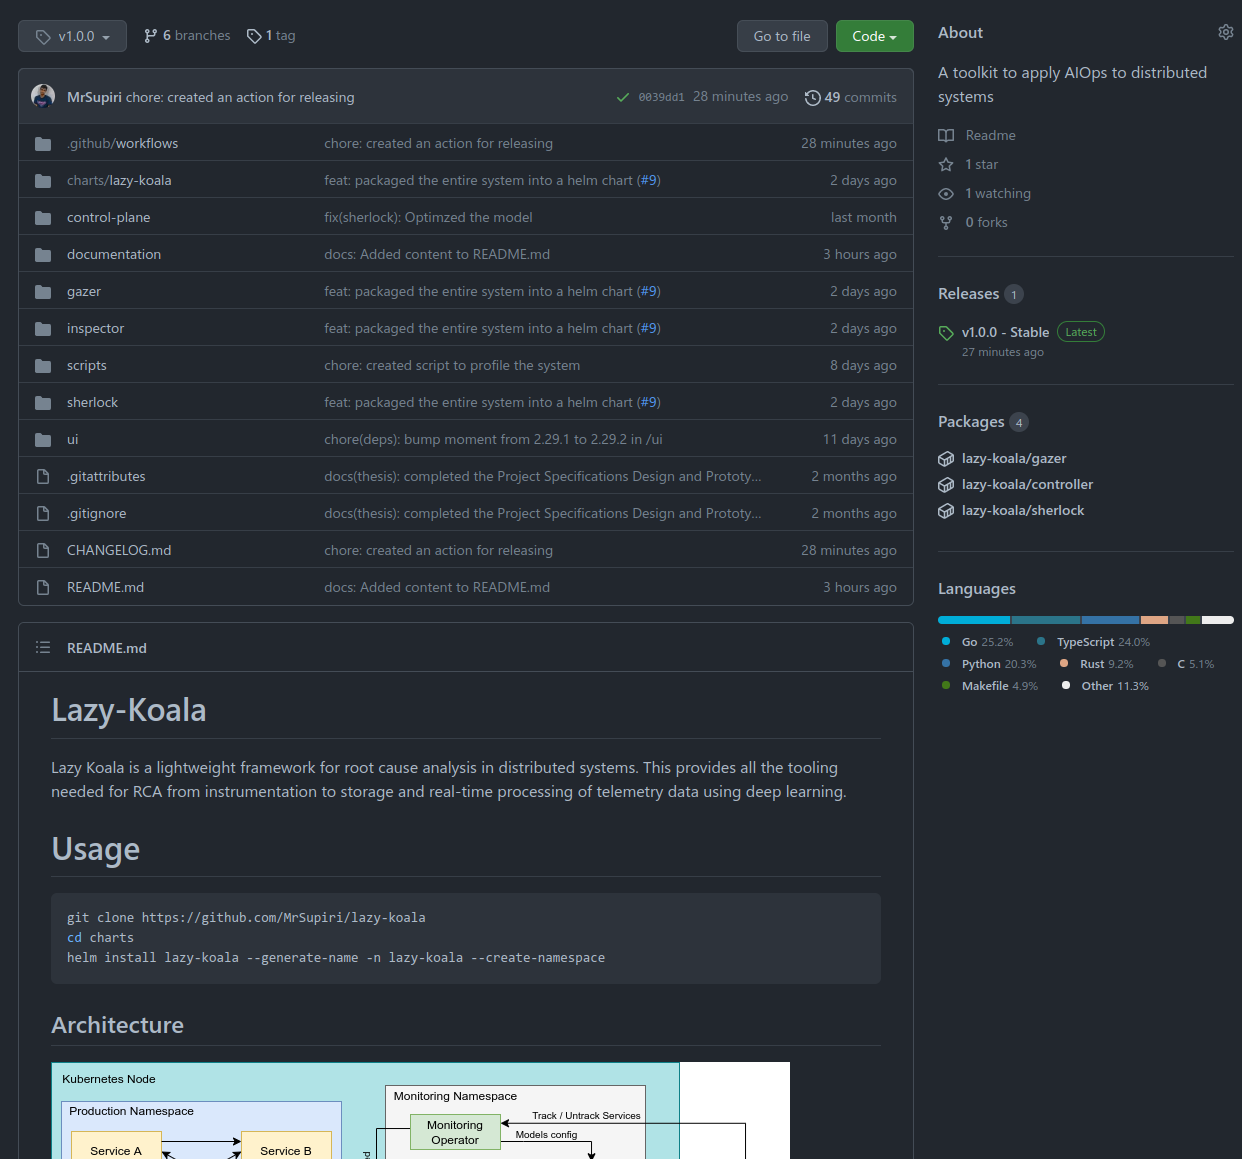
\includegraphics[width=16.5cm]{assets/appendix/github.png}
    \caption{Github Repository Structure (self-composed)}
\end{figure}

\newpage

\section{Conventional Commits}

Conventional commits allow both humans and machines to easily understand the changes made to the code. It starts with and tag which indicates the type of change made. Following that the scope of the commit specifies which part of the code base code changed. Finally, the commit message is used to describe the change \citep{Conventi55:online}.

\begin{figure}[H]
    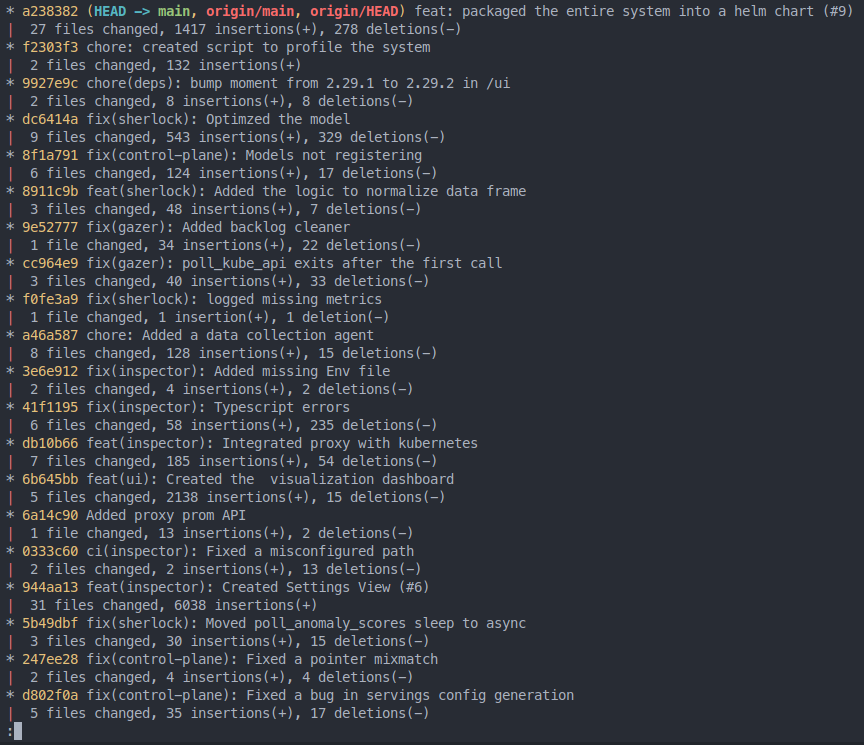
\includegraphics[width=16.5cm]{assets/appendix/commits.png}
    \caption{Use of Semantic Commits (self-composed)}
\end{figure}


\section{Continuous Integration \& Continuous Delivery Pipeline}

\begin{figure}[H]
    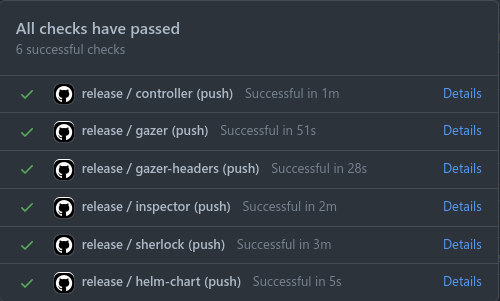
\includegraphics[width=16.5cm]{assets/appendix/ci.png}
    \caption{Continuous Integration \& Continuous Delivery Pipeline (self-composed)}
\end{figure}

\section{Release Note}


\begin{figure}[H]
    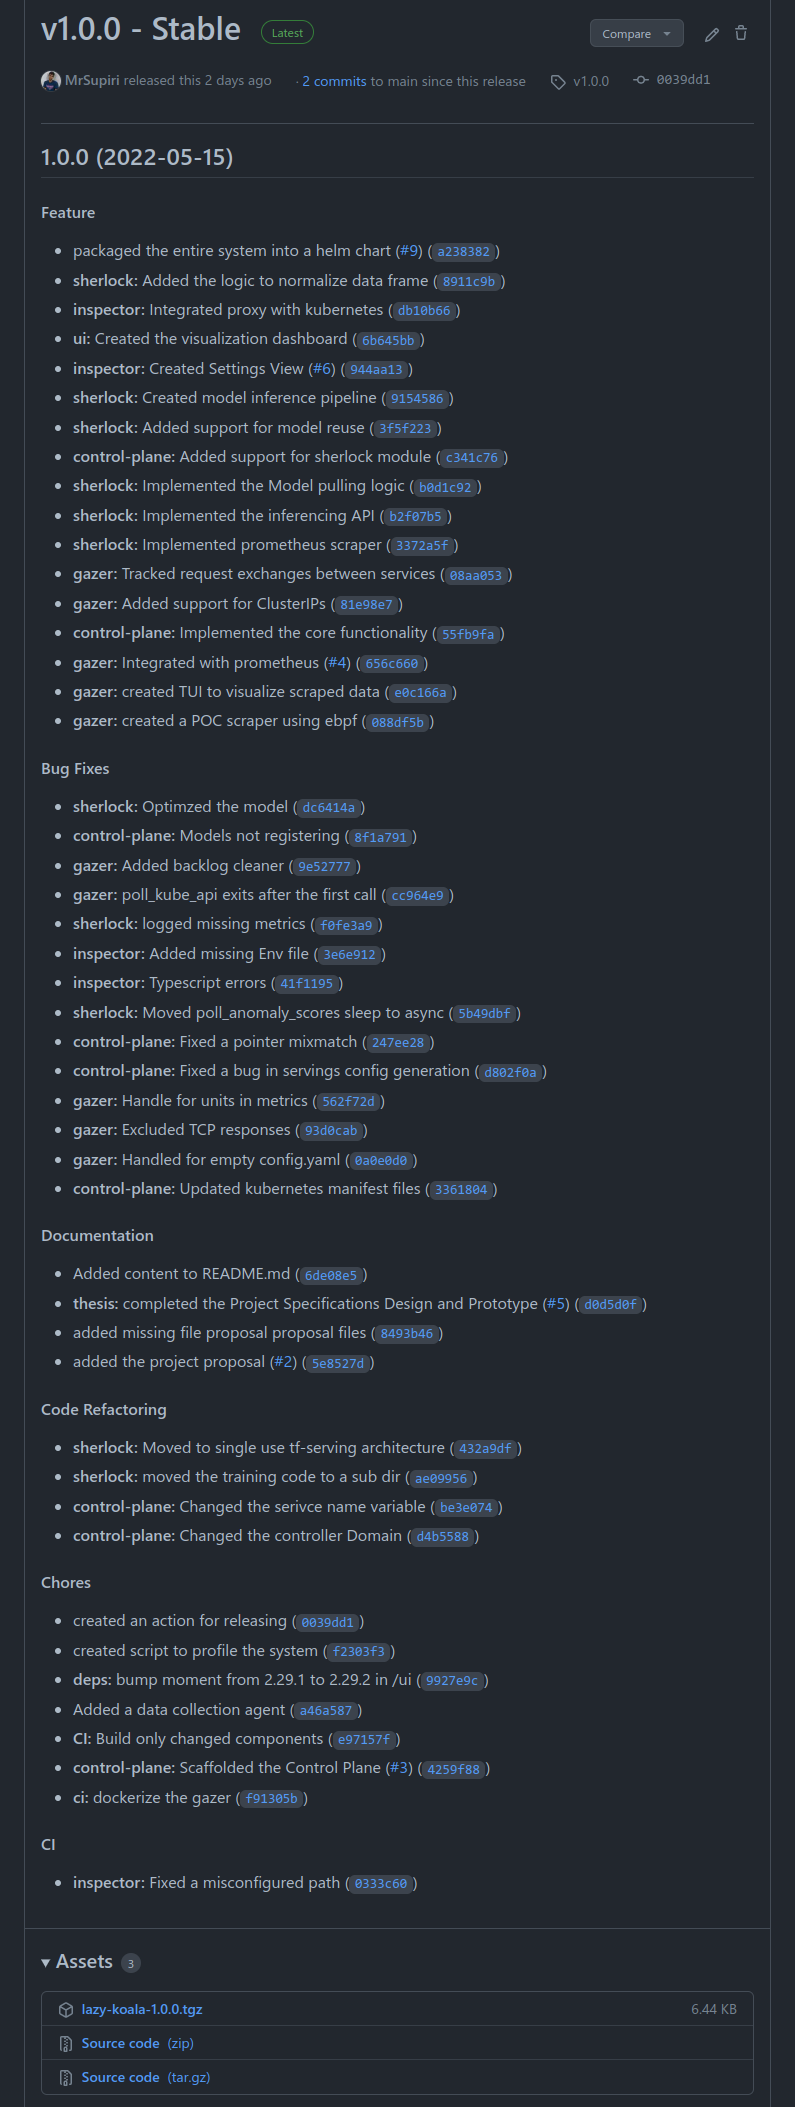
\includegraphics[height=22.5cm]{assets/appendix/release.png}
    \caption{Generated release note from the commit history (self-composed)}
\end{figure}
